% intro %
\subsection{Introduction}
When particles collide at high energies inside a particle detector, the collision products either decay into stable particles or simply do not interact with the detector.
In order to identify the original decay products coming out of the collision, we need a way to reconstruct them from the detector signals.
The CMS experiment can achieve this using a holistic approach developed by the ALEPH experiment at LEP called particle flow (PF).

This algorithm uses the various signals captured by the CMS subdetectors, as shown in Fig.~\ref{fig:Particles_in_CMS}, %PF_nature_detector),
in order to reconstruct physics objects such as muons, electrons, photons, jets, taus, and missing transverse energy, which are used later in physics analyses.
This section provides a description of the PF algorithm and its process for forming energy clusters from energy deposits in the calorimeters.
Additionally, calorimeter cluster calibration using the conventional method is covered (fix me).

\begin{figure}[t!]
\centering
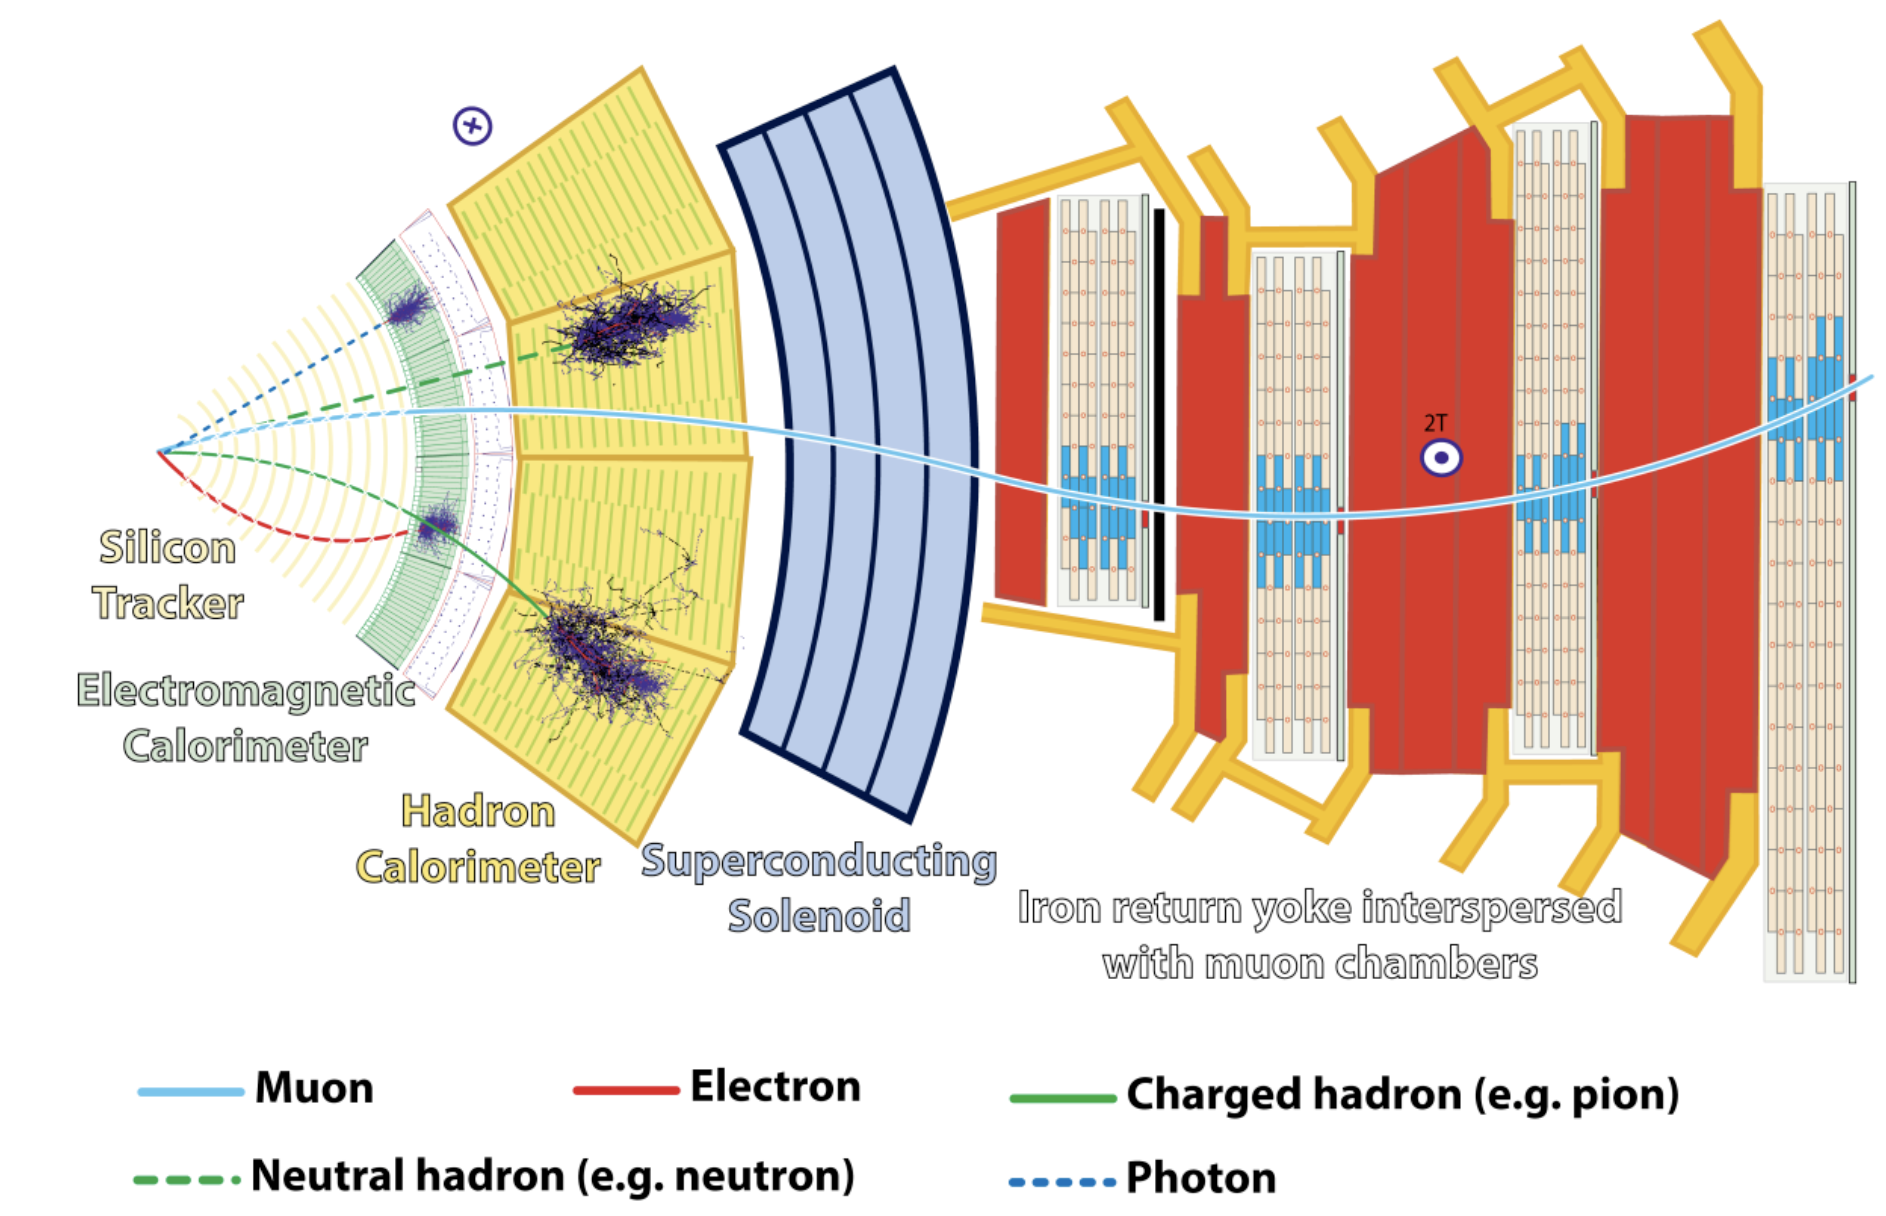
\includegraphics[width=0.99\textwidth]{figures/particles_signture_in_detector.png}
\caption[Transverse view of the CMS detector]{Particles signture in detector. Figure source~\cite{PF}.}
\label{fig:Particles_in_CMS}
\end{figure}

\subsection{Particle Flow Algorithm}
The PF algorithm aims to reconstruct and identify all the final particles produced in an event by utilizing the fact that different particles leave different signatures in the CMS subdetectors as shown in Fig~\ref{fig:PF_diagram}. %cms_particle_signtures).
The PF algorithm in CMS operates in two different modes: online PF, which is used during data collection to select interesting events, and offline PF, which is utilized after data collection for detailed offline data analyses. %source for PF and HLT).

\begin{figure}[t!]
\centering
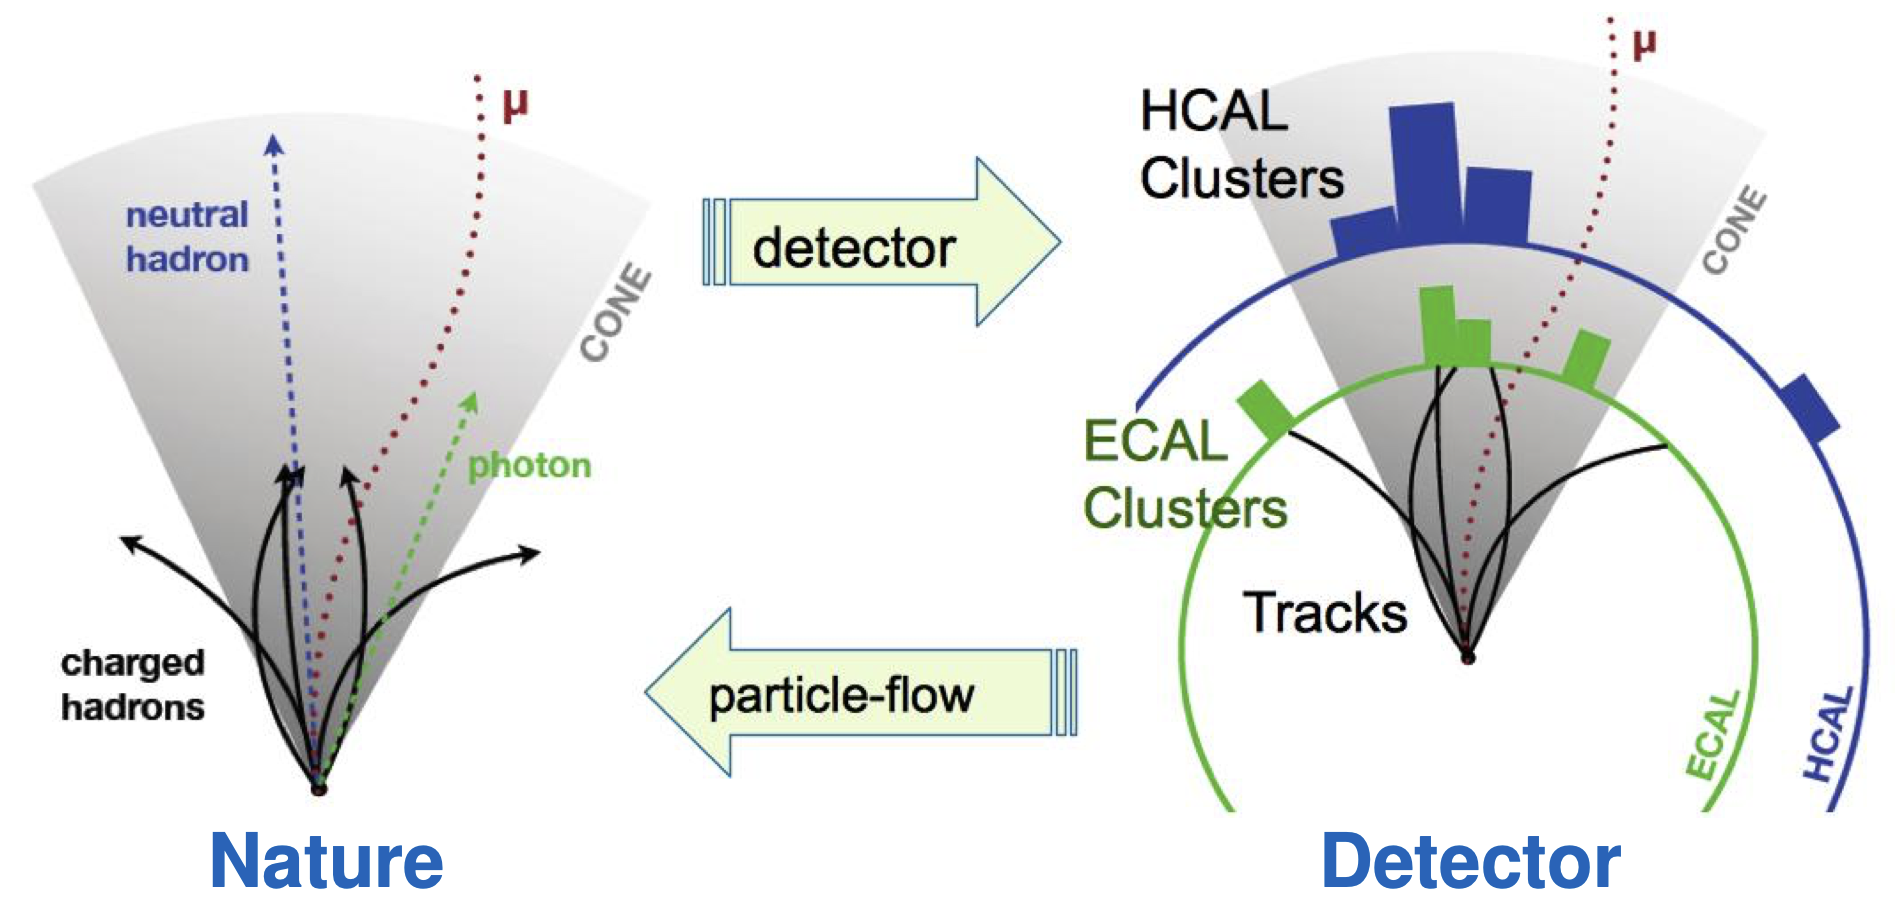
\includegraphics[width=0.99\textwidth]{figures/PF.png}
\caption[A diagram of the PF algorithm]{The CMS Particle Flow algorithm combines sub-detector information and reconstructs individual
particles in collision events for converting detector signals back to physical objects. Figure source~\cite{PF_diagram}.}
\label{fig:PF_diagram}
\end{figure}

The PF algorithm follows these steps (source):
First, the PF algorithm reconstructs essential elements which are charged particle tracks and calorimeter energy clusters.
Details of the clustering algorithm and the cluster calibration will be discussed later in this chapter.
Second, it links these PF elements based on their spatial proximity in $\eta$-$\phi$ space.
The linking order is: track $\rightarrow$ ECAL cluster $\rightarrow$ HCAL cluster.
%The linking rule here is to connect small elements to the bigger ones, meaning they must be touching in the eta-phi space.
%The order of the elements is from small to big: track, ECAL cluster, and HCAL cluster.
%Examples of links between the elements are: tracks and ECAL clusters, tracks and HCAL clusters, and an inner tracks and muon tracks.
%After all the established links, the PF blocks contain groups of linked tracks and clusters.
%Any left elements, such as a single track or a cluster,  their own blocks.
Examples of linked elements include tracks and ECAL clusters, tracks and HCAL clusters, and inner tracks and muon tracks.
Once all connections are established, PF blocks are formed, consisting of groups of linked tracks and clusters.
Any unlinked elements, such as isolated tracks or clusters, form their own separate blocks.

%Third, a list of PF particle candidates which follows a strict order, starting with the cleanest signature in the CMS muons.
%Then, isolated electrons and photons.
%After that, neutral hadrons and non-isolated photons.
%Lastly, everything left is charged hadrons.
Third, the algorithm reconstructs a list of PF particle candidates in a hierarchical order, beginning with the cleanest signatures in CMS:
Muons are identified first, followed by isolated electrons and photons. Next, neutral hadrons and non-isolated photons are reconstructed.
Finally, any remaining particles are classified as charged hadrons.
For charged hadrons, the energy is determined by comparing the cluster energy sum to the track momenta sum.
Additionally, any isolated tracks are reconstructed as charge hadrons.

\subsection{Calorimeter Clustering}
\label{subsec:clustering}
The clustering algorithm used in the PF computes the cluster positions and their energies.
This algorithm is done separately in each calorimeter through multiple steps.
First, we identify topological clusters by looking for a group of calorimeter cells with energy deposits above a certain threshold, and they must share at least one neighbor.
%The threshold values could be viewed in Fig.~\ref{fig:seeds}.
Next, we identify any calorimeter cell, or seed whose energy is a local maximum with respect to its immediate neighbors.
Different configurations of cluster seeds are shown in Fig.~\ref{fig:seeds}.
Each topological cluster could have one seed or multiple as shown in Fig.~\ref{fig:topo_cluster}.

\begin{figure}[t!]
\centering
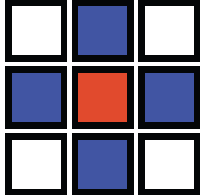
\includegraphics[width=0.25\textwidth]{figures/seed_4neighbours.png}
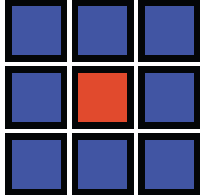
\includegraphics[width=0.25\textwidth]{figures/seed_8neighbours.png}
\caption[Types of cluster seed]{Different types of seeds. Figure source~\cite{Clustering}.}
\label{fig:seeds}
\end{figure}

\begin{figure}[t!]
\centering
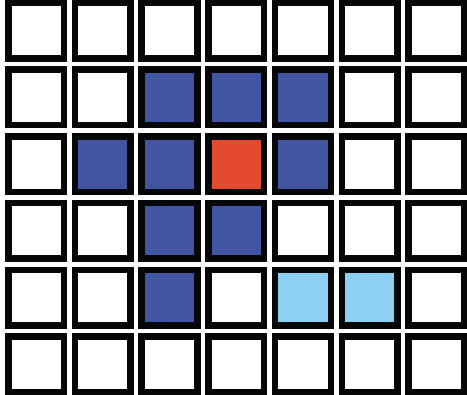
\includegraphics[width=0.25\textwidth]{figures/topological_cluster_oneseed.png}
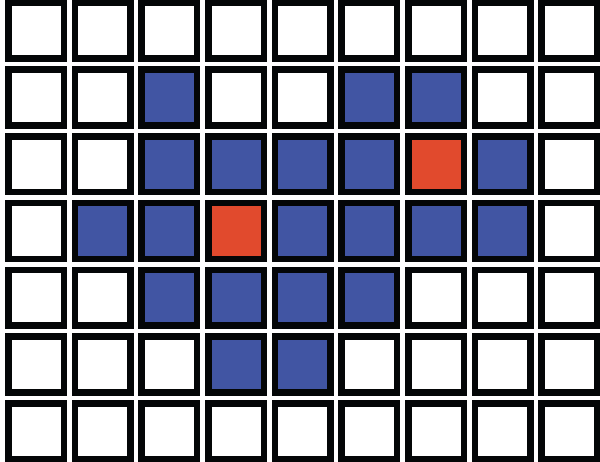
\includegraphics[width=0.25\textwidth]{figures/topological_cluster_many_Seeds.png}
\caption[Types of topological cluster]{Types of topological cluster. Figure source~\cite{Clustering}.}
\label{fig:topo_cluster}
\end{figure}

Lastly, we compute the cluster positions and energies.
In the single-seed case, the cluster energy will be the sum of all the individual cell energies within the cluster, and its position will be the energy-weighted average of the individual cell positions.
However, for the multiple-seed case, each seed is assumed to represent a unique energy cluster and the energy deposited in non-seed cells will be shared between the various clusters within the topological cluster.
Here the cluster energies and positions are determined using an iterative procedure based on the energy-weighted averages of fractional cell energies as shown in Fig.~\ref{fig:clustering}. (source)

\begin{figure}[t!]
\centering
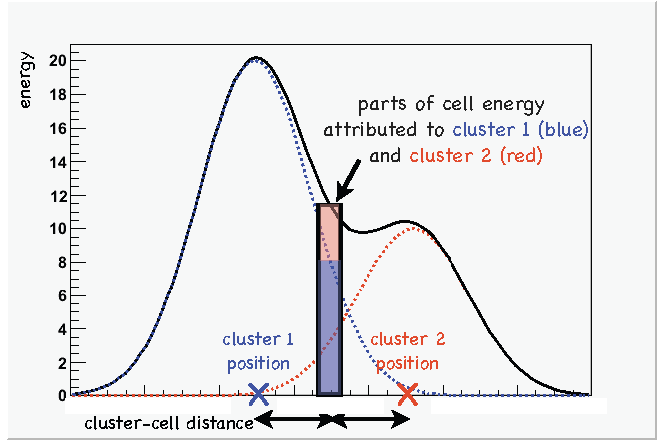
\includegraphics[width=0.50\textwidth]{figures/energy_sharing.png}
\caption[Energy shared between clusters]{Energy shared between clusters. Figure source~\cite{Clustering}.}
\label{fig:clustering}
\end{figure}

\subsection{Calorimeter Cluster Calibration}
As mentioned in the PF algorithm section, photons, and neutral hadrons are reconstructed only from calorimeter clusters.
Neural particles could have a clear signature, where a calorimeter cluster separated from any charged particle track or will overlap with a charged particle cluster.
In the second case, the energy deposits of the neutral particles are the excess energy with respect to the sum of the associated charged particle momenta. Therefore, proper calibration of the calorimeter response to photons and hadrons will enhance particle identification and reduce the likelihood of misreconstructed energy excess.
The following sections describe the calibration of electromagnetic and hadron clusters.


\subsubsection{Electromagentic deposits}

In the clustering algorithm, several thresholds are applied to the ECAL cell energies %(fig).
As a consequence, the energy measured in the clusters is expected to be smaller than the actual energy of the incoming photons, especially at low energy.
Therefore, a calibration is required to account for the effects of the thresholds.
This calibration is applied to all ECAL clusters before the hadron cluster calibration is done and before the particle identification step.

This residual energy calibration uses a large sample of photons with varied energy ranges.
Only photons that do not experience photon conversion (pair production) prior to the entrance in the ECAL are considered to deal with the calibration of a single cluster.
Similar to clustering, the correction of ECAL energy clusters is applied separately in each region of the ECAL.

For the barre region, the Analytical function f(E,$\eta$) = g(E)h($\eta$), where E is the energy and $\eta$ is the pseudorapidity of the cluster, is fitted to each $E^{true}$ bin's ratio distribution of ($E^{true}$ / E).
By reconstruction this function, the residual correction (correction factor) to be applied to the measured cluster energy (E) is close to unity at high energy, where threshold effects vanish.

$E_{calib} = \alpha(E^{true},\eta^{true})E_{ECAL} + \beta(E^{true},\eta^{true})[E_{PS1}+\gamma(E^{true},\eta^{true})E_{PS2}]$

The endcap regions' calibrated cluster energy is expressed as in previous eq. The calibration parameters (numerical value) $\alpha$, $\beta$, and $\gamma$ are chosen in each ($E^{true}$,$\eta^{true}$) bin to minimize the $\chi^{2}$ value. The $\chi^{2}$ measures the discrepancy between observed and expected values. The smaller the value, the better fit of function between the data and the model.



$\chi^{2}$ equation (add equation number):

$\chi^2 = \sum_{i=1}^{N_{events}}\frac{(E_{i}^{calib} - E_{i}^{true})}{\sigma_{i}^{2}}$


\subsubsection{Hadron deposits}

Hadrons generally deposit their energies in the ECAL and HCAL.
As described in the previous section, the ECAL has already been calibrated for photons.
However, the ECAL has a different energy response to hadrons.
The calibrated calorimeter energy associated with a hadron is expressed as in eq()

Using a large sample of simulated neutral hadron, the calibration coefficients $a$, $b$, $c$, and the functions $f$ and $g$ are determined using $\chi^{2}$ method, which was described previously, 

hadrons equation(add eq number):

$E_{calib} = a + b(E)f(\eta)E_{ECAL} + c(E)g(\eta)E_{HCAL}$ %for hadrons
